\documentclass{article}

% Pacotes
\usepackage[english]{babel}
\usepackage[letterpaper,top=2cm,bottom=2cm,left=3cm,right=3cm,marginparwidth=1.75cm]{geometry}
\usepackage{amsmath}
\usepackage{graphicx}
\usepackage[colorlinks=true, allcolors=blue]{hyperref}
\usepackage{listings}
\usepackage{amssymb}
\usepackage{here}

\title{EP 2}
\author{Gabriel Delvaje Corrêa - 9370330}

\begin{document}
\maketitle

\section{Introdução}

Este relatório visa determinar o número de simulações necessárias para alcançar um erro de 0.005 na aproximação da integral da função \(f(x) = e^{-(ax)} \cos(bx)\) utilizando quatro métodos de Monte Carlo: Crude, Hit or Miss, Importance Sampling e Variate Control. Essa análise busca fornecer uma compreensão clara da eficácia de cada método em termos de precisão, permitindo uma escolha informada do método mais apropriado para alcançar a precisão desejada. 

\section{Gerando números aleatórios em Python}

Em Python, pode-se importar a biblioteca \verb|random| que oferece funcionalidades para gerar números aleatórios. 

\subsection{Uniforme}

Pode-se usar a função \verb|random.uniform(a, b)| onde \verb|a| é o limite inferior do intervalo e \verb|b| é o limite superior. 

\subsection{Beta}

Pode-se gerar números aleatórios seguindo a distribuição beta usando a função \verb|numpy.random.beta(a, b, size)|, onde \verb|a| e \verb|b| são parâmetros da distribuição e \verb|size| é o tamanho da amostra a ser gerada. 

\subsection{Gama}

Para gerar números aleatórios seguindo a distribuição gama em Python, usamos a função \verb|numpy.random.gamma(shape, scale, size)|, onde \verb|shape| é o parâmetro alfa da distribuição, \verb|scale| é o inverso do parâmetro beta e \verb|size| é o tamanho da amostra.  

\subsection{Weirbull}

Para gerar números aleatórios seguindo a distribuição Weibull em Python, usamos a função \verb|numpy.random.weibull(a, size)|, onde \verb|a| é o parâmetro alfa da distribuição e \verb|size| é o tamanho da amostra.

\section{Simulações de Monte Carlo}

\subsection{Monte Carlo Cru}

Para integrar uma função qualquer \( f(x) \) no intervalo \([a, b]\) usando amostragem de variáveis aleatórias uniformemente distribuídas \( X_i \sim \text{U}[a, b] \), pode-se empregar a seguinte abordagem:

\[ \bar{I} = \frac{1}{n} \sum_{i=1}^{n} f(X_i) \]

onde \( \bar{I} \) é a estimativa da integral e \( \mathbb{E}(\bar{I}) \) é a sua esperança. Sabe-se que esta estimativa é não enviesada, ou seja, \( \mathbb{E}(\bar{I}) = I \), onde \( I \) é a integral real de \( f(x) \) no intervalo \([a, b]\). 

Para integrar a função \(f(x)=e^{-(ax)}\cos(bx)\) no intervalo \([0, 1]\), em que \(a = 0.426358491\) e \(b = 0.39128791843\), será utilizado:

\[ \bar{I} = \frac{1}{n} \sum_{i=1}^{n} e^{-(ax_i)}\cos(bx_i) \]

Para ter uma ideia de como essa somatória se comporta conforme \(n\) aumenta, foi executada a mesma somatória para \(0 < n < 500\).

\begin{figure}[H]
    \centering
    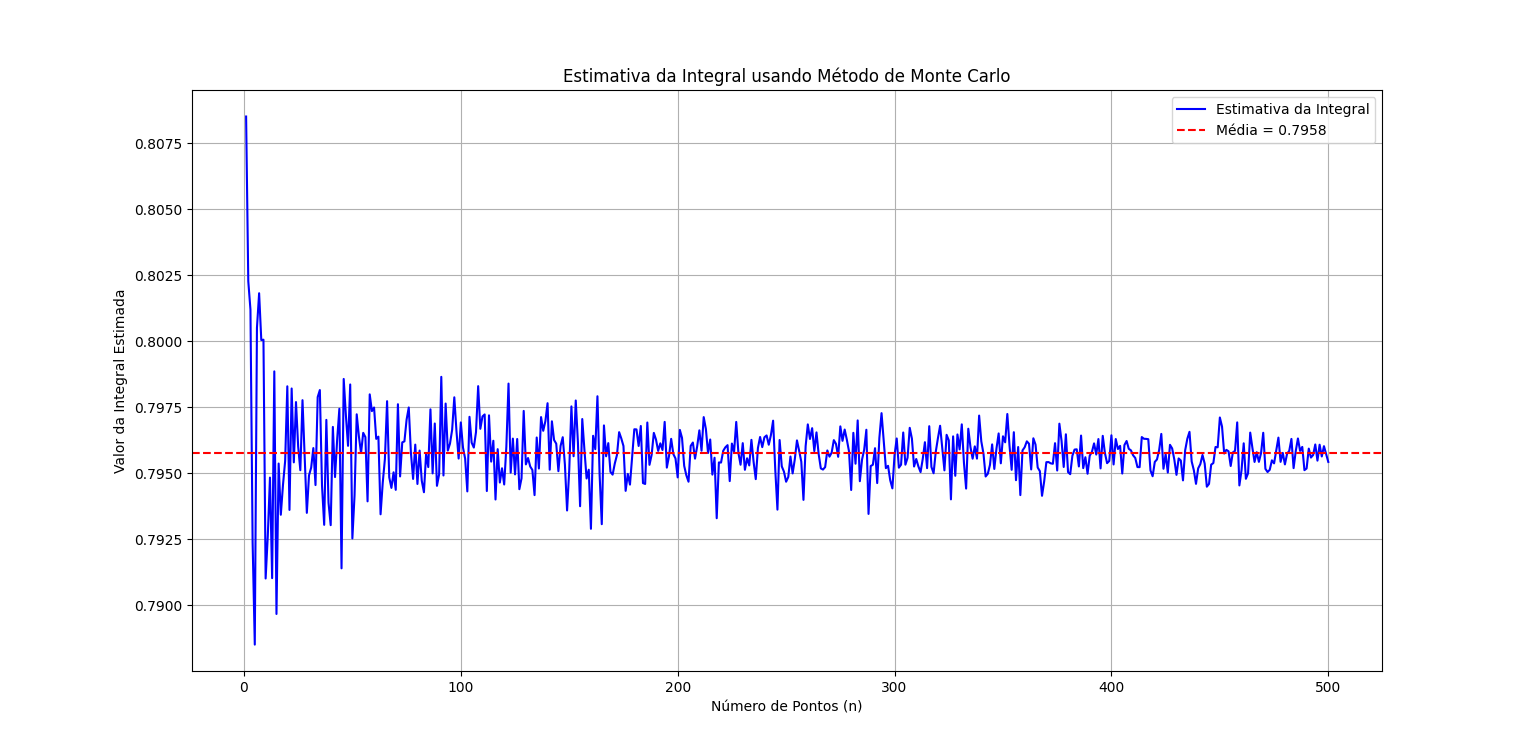
\includegraphics[width=0.75\linewidth]{estimativa integral de 1 a 500.png}
\end{figure}

A linha tracejada informa a média. É possível ver que, conforme \(n\) aumenta, os valores da somatória se aproximam da média, ou seja, a variância diminui.

Isso posto, o código foi executado 100 vezes para \(n = 500\), gerando uma amostra que foi plotada no histograma a seguir.

\begin{figure}[H]
    \centering
    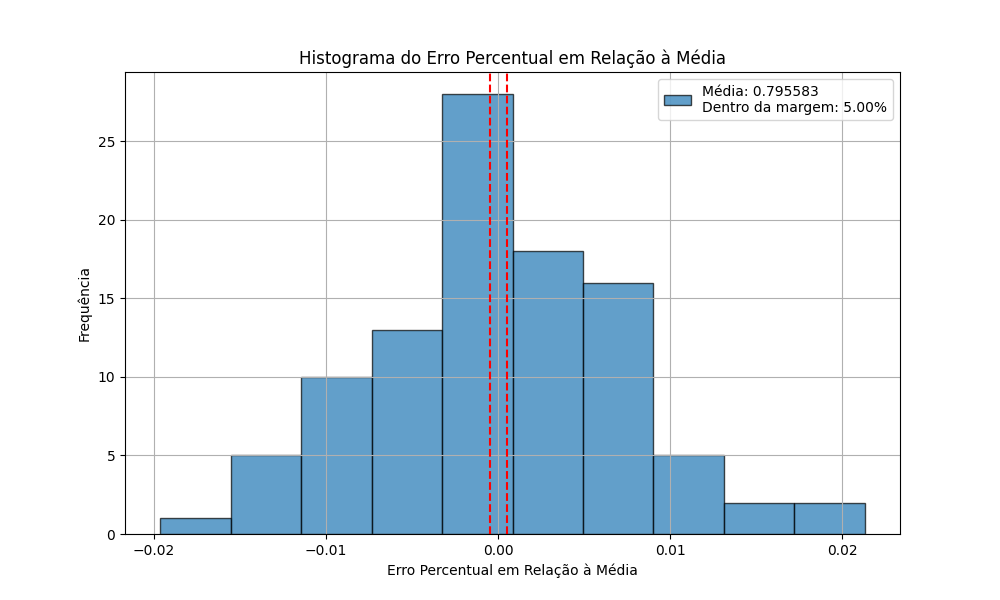
\includegraphics[width=0.75\linewidth]{cru 500.png}
\end{figure}

Observa-se que para essa simulação apenas 5 por cento da amostra ficou dentro da margem de erro de 0.005.

Aumentando \(n\) e plotando no histograma, chegou-se a \(n = 900000\) para esse método, que, nas simulações feitas, respeitou bem a quantidade da amostra dentro da margem de erro procurada.

\begin{figure}[H]
    \centering
    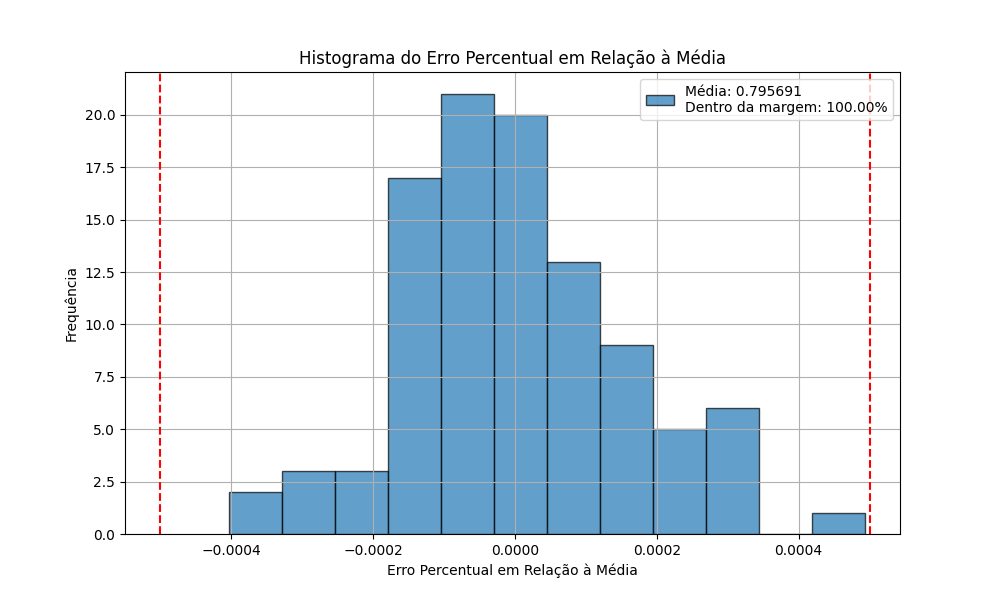
\includegraphics[width=0.75\linewidth]{cru 900000.png}
\end{figure}

\subsection{Monte Carlo Hit ou Miss}

Para esse método, para integrar uma função qualquer \( f(x) \) no intervalo \([a, b]\) usando amostragem de variáveis aleatórias uniformemente distribuídas \( X_i,Y_i \sim \text{U}[a, b] \), pode-se empregar a seguinte abordagem:

\[ \bar{I} = \frac{1}{n} \sum_{i=1}^{n} h(X_i,Y_i) \]

em que \(h(x,y) = \text{ind}(y \leq f(x))\), ou seja, ao sortear os pontos, ele é computado na somatória apenas se cair dentro da curva produzida por \(f(x)\).

Isso posto, produziu-se o mesmo histograma para esse método com \(n = 900000\):

\begin{figure}[H]
    \centering
    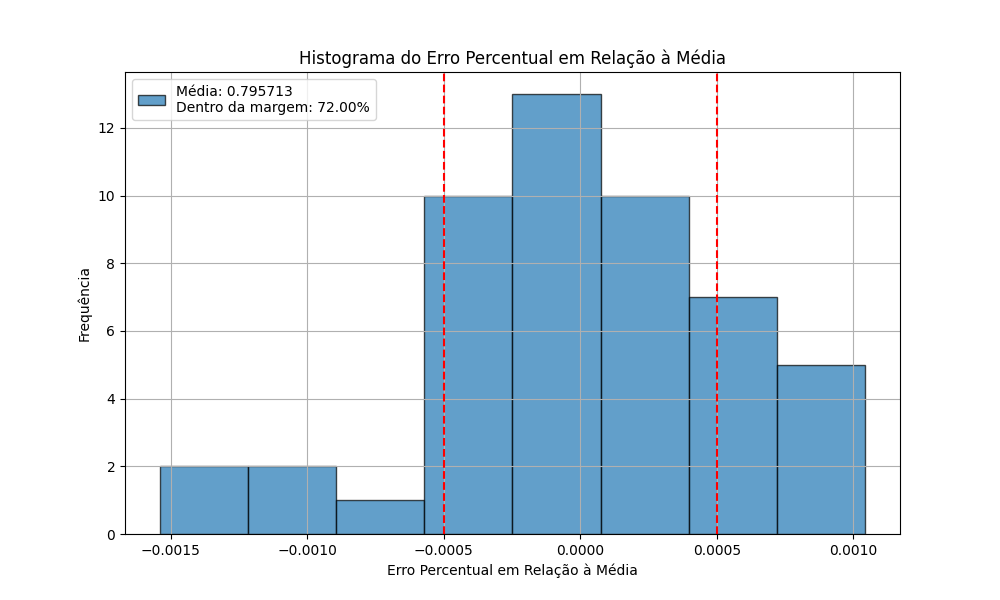
\includegraphics[width=0.75\linewidth]{hit 900000.png}
\end{figure}

No entanto, a porcentagem da amostra dentro da margem de erro não foi satisfatória. Aumentando \(n\), chegou-se a \(n = 9000000\), que demonstrou uma porcentagem satisfatória da amostra dentro da margem, como mostrado a seguir:

\begin{figure}[H]
    \centering
    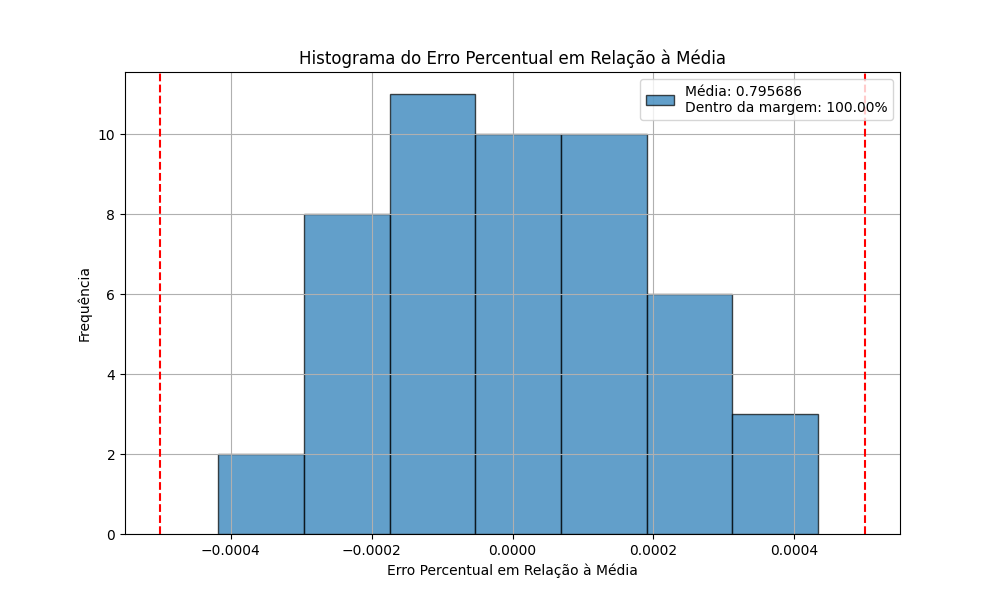
\includegraphics[width=0.75\linewidth]{hi 9 milhoes.png}
\end{figure}

\subsection{Amostragem por Importância}

Nesse método, para integrar uma função qualquer \( f(x) \) no intervalo \([a, b]\) é preciso escolher uma função de densidade para a amostragem de variáveis aleatórias  \( X_i \sim g(x) \). Desse modo, pode-se empregar a seguinte abordagem:

\[ \bar{I} = \frac{1}{n} \sum_{i=1}^{n} \frac{f(X_i)}{g(X_i)} \]

A função de densidade escolhida foi a Beta, por gerar pontos aleatórios no intervalo \([0,1]\) distribuídos não uniformemente.

Para a escolha dos parâmetros \(\alpha\) e \(\beta\), foi produzido um código para testá-los e plotar em gráfico a curva gerada, como também a curva da função \(f(x)\) procurada e a razão entre as duas.

\begin{figure}[H]
    \centering
    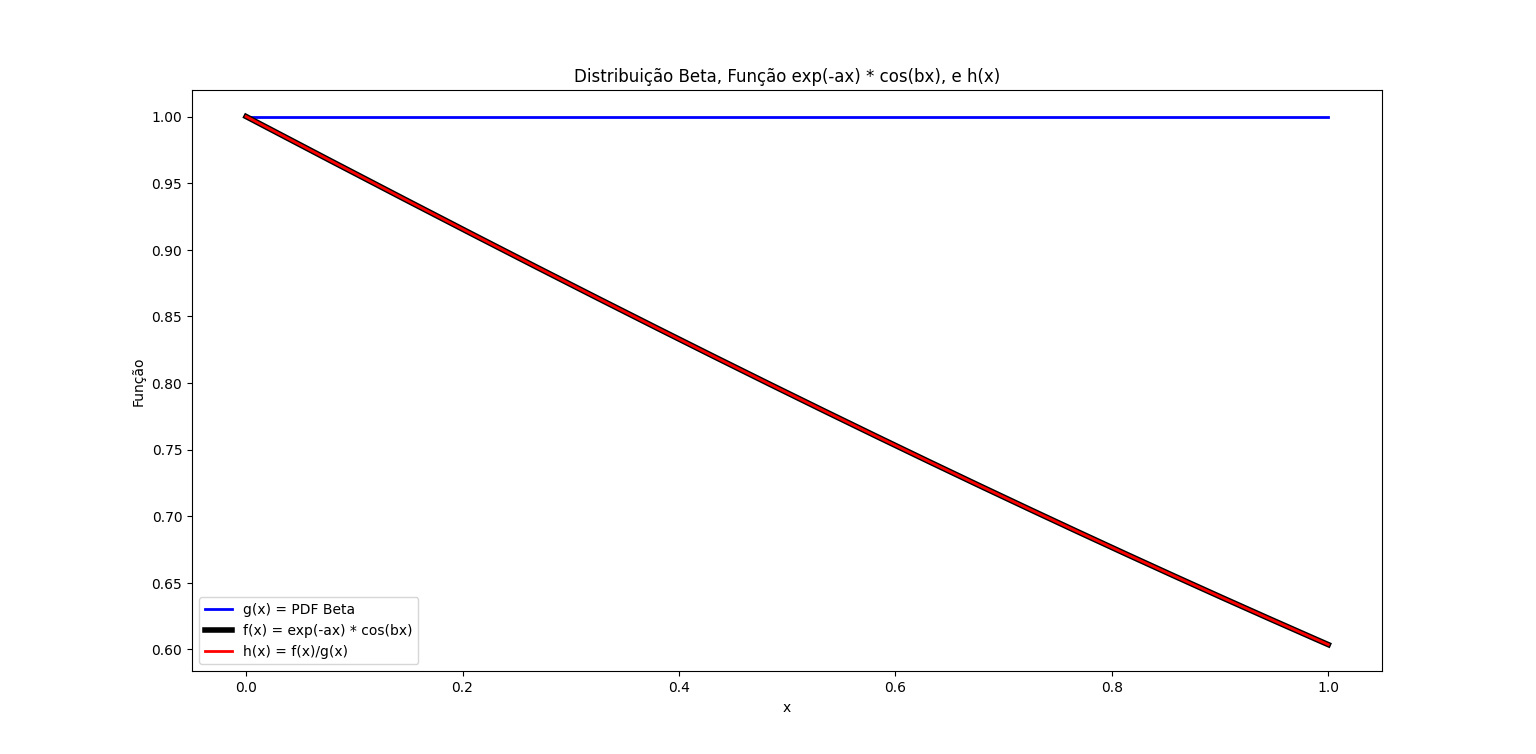
\includegraphics[width=0.75\linewidth]{escolha de beta.png}
\end{figure}

Os parâmetros que melhor se ajustaram foram \(\alpha = 1\) e \(\beta = 1\). Assim, a somatória resultou em:

\[ \bar{I} = \frac{1}{n} \sum_{i=1}^{n} \frac{e^{-(ax)}\cos(bx)}{\frac{x^{\alpha - 1}(1-x)^{\beta-1}}{B(\alpha,\beta)}} \]

Substituindo os parâmetros escolhidos, a somatória se torna:

\[ \bar{I} = \frac{1}{n} \sum_{i=1}^{n} e^{-(ax)}\cos(bx)B(\alpha,\beta) \]

Foi, então, gerado um histograma com \(n = 900000\), que gerou uma porcentagem dentro da margem satisfatória nas simulações executadas.

\subsection{Variável de Controle}

Nesse método, para integrar uma função qualquer \( f(x) \) no intervalo \([a, b]\) é preciso escolher uma função polinomial \(g(x)\) que se assemelha a \(f(x)\) e gerar pontos aleatórios, a distribuição escolhida foi \( X_i \sim \text{U}[a, b] \). Desse modo, pode-se empregar a seguinte abordagem:

\[ \bar{I} = \frac{1}{n} \sum_{i=1}^{n} f(X_i) - g(X_i) + g', \]

onde \( g' = \int_{a}^{b} g(x) \).

Para a escolha da função polinomial, \(f(x)\) foi plotado em gráfico. A partir disso, observou-se que a curva no intervalo\([0,1]\) se assemelha a uma reta.

\begin{figure}[H]
    \centering
    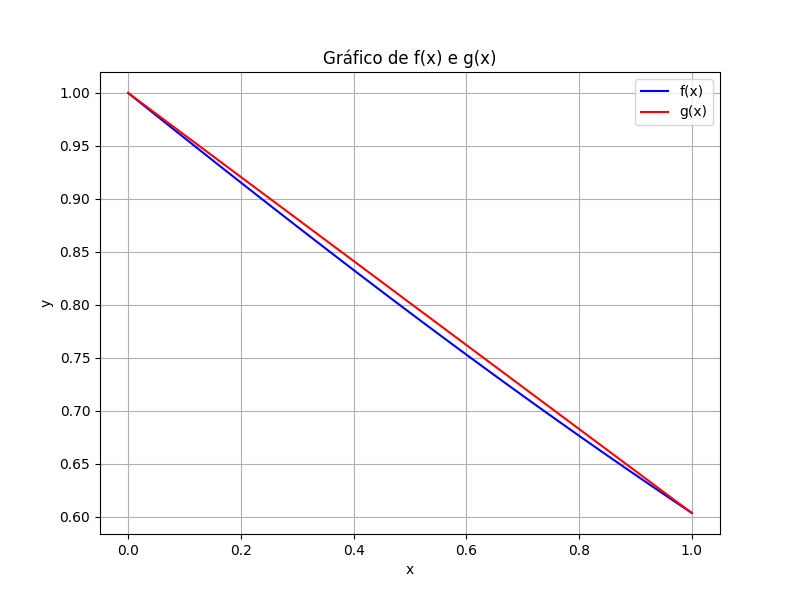
\includegraphics[width=0.75\linewidth]{reta.png}
\end{figure}

Assim, a reta \(g(x) = -0.394634796444x + 1\) foi escolhida. Portanto,

\[ g' = \int_{0}^{1} -0.394634796444x + 1 \]

\[ g' = -0.394634796444\frac{x^{2}}{2} + x\big|_{0}^{1} \]

\[ g' = 0.801768260178 \]

Assim, temos a somatória:

\[ \bar{I} = \frac{1}{n} \sum_{i=1}^{n} e^{-(aX_i)}\cos(bX_i) + 0.3946X_i - 0.1982 \]

Para esse método, foi necessário \(n = 500\) para uma porcentagem mais que satisfatória dentro da margem.

\begin{figure}[H]
    \centering
    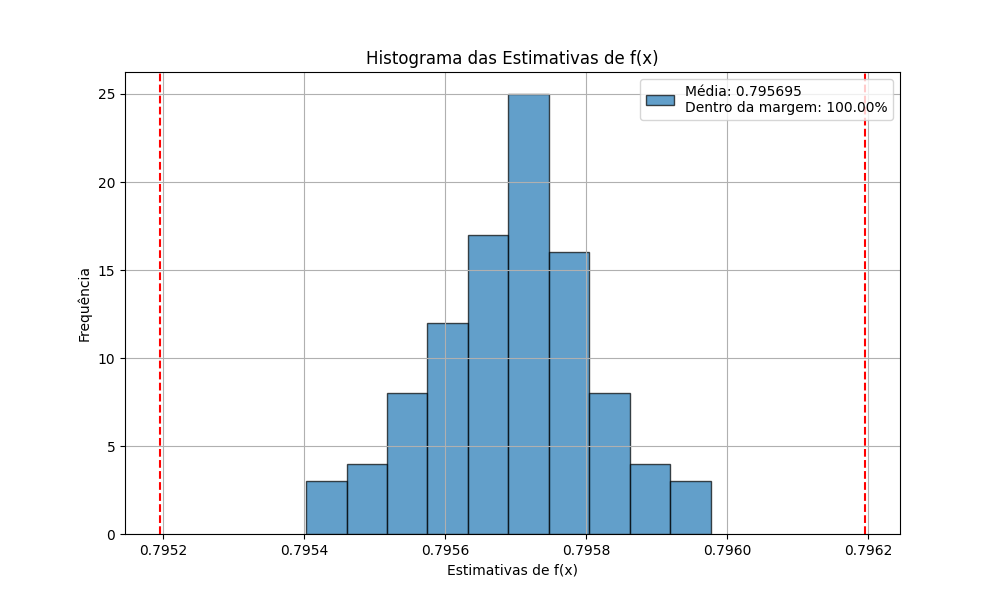
\includegraphics[width=0.75\linewidth]{control.png}
\end{figure}

\section{O programa}

O código cria quatro classes, uma para cada método. Após definir as classes que implementam os diferentes métodos de Monte Carlo para estimar integrais, o código instancia cada uma dessas classes com os parâmetros relevantes, como o intervalo de integração e quaisquer parâmetros adicionais necessários para cada método específico.

Em seguida, o código executa múltiplas simulações para cada método, calculando as estimativas da integral. Isso é feito chamando o método \verb|estimate_integral| de cada instância das classes.

Depois de calcular as estimativas, o código calcula as médias e desvios padrão das estimativas para cada método. Esses valores são então usados para plotar a distribuição das estimativas e calcular a porcentagem de pontos dentro de uma margem de erro especificada.

Além disso, o código calcula os erros relativos das estimativas em relação às médias calculadas. Isso permite avaliar a precisão de cada método em relação à média das estimativas.

Finalmente, o código gera um gráfico comparativo, aproximando de curvas normais, das distribuições das estimativas para cada método, adicionando linhas tracejadas verticais para indicar a margem de erro. O gráfico é exibido juntamente com os valores de média e variância calculados para cada método.

Por fim, o código exibe o tempo decorrido para realizar os cálculos.

Em resumo, o código implementa e compara diferentes métodos de Monte Carlo para estimar integrais, fornecendo uma análise visual e quantitativa de suas eficácias em termos de precisão e eficiência computacional.

Exemplo:

\begin{figure}[H]
    \centering
    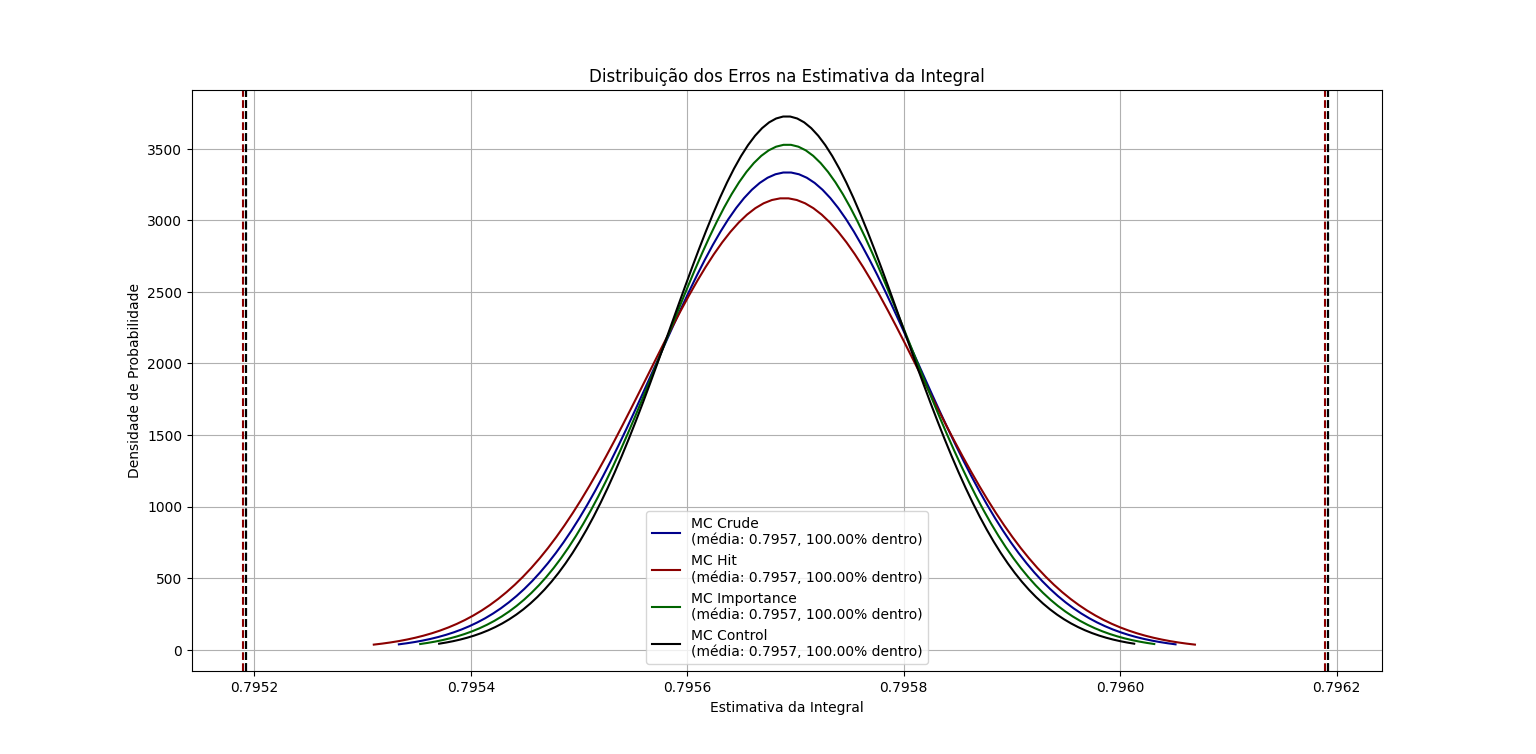
\includegraphics[width=0.75\linewidth]{ep 2.png}
\end{figure}

Monte Carlo Crude:

- média: 0.7957

- variância: 0.0001

Monte Carlo Hit or Miss:

- média: 0.7957

- variância: 0.0001

Monte Carlo Importance Sample:

- média: 0.7957

- variância: 0.0001

Monte Carlo Control Variate:

- média: 0.7957

- variância: 0.0001

Tempo decorrido para cálculo: 61.94 segundos

\end{document}
